\clearpage
\section{Fully Dressed Use Cases}

This section presents detailed fully dressed use cases following the Cockburn format.

\subsection{UC-01: Generate Sprite (Fully Dressed)}

\noindent
\begin{minipage}{\textwidth}
\centering
\captionof{table}{Fully Dressed Use Case: Generate Sprite}
\label{tab:uc_sprite_full}
\small
\begin{tabular}{|p{3cm}|p{9.5cm}|}
\hline
\textbf{Use Case ID} & UC-01 \\
\hline
\textbf{Use Case Name} & Generate Sprite \\
\hline
\textbf{Scope} & Pixelar Web Application \\
\hline
\textbf{Level} & User Goal \\
\hline
\textbf{Primary Actor} & Authenticated User \\
\hline
\textbf{Stakeholders} & 
\textbf{User}: Wants high-quality sprite images. \newline
\textbf{System}: Process requests efficiently. \newline
\textbf{AI Provider}: Receive well-formed requests. \\
\hline
\textbf{Preconditions} & 
1. User authenticated with active session \newline
2. User has credits OR valid BYOK API key \newline
3. AI provider services available \\
\hline
\textbf{Success Guarantee} & 
1. Sprites generated and displayed \newline
2. Images uploaded to blob storage \newline
3. Metadata saved to database \newline
4. Credits deducted (if using platform key) \\
\hline
\textbf{Main Success Scenario} & 
1. User navigates to Sprite Generator \newline
2. User selects sprite type (Character/Object) \newline
3. User enters text prompt \newline
4. User configures parameters (style, viewpoint, ratio, colors) \newline
5. User clicks ``Generate'' \newline
6. System validates credits/BYOK \newline
7. System constructs optimized prompt \newline
8. System calls AI provider \newline
9. System uploads and saves images \newline
10. System displays sprites \newline
11. User downloads or saves to project \\
\hline
\textbf{Extensions} & 
\textbf{6a.} Insufficient credits: Display error \newline
\textbf{8a.} Provider unavailable: Switch to fallback \newline
\textbf{8b.} Policy violation: Ask to modify prompt \newline
\textbf{9a.} Timeout: Cancel, no credits deducted \\
\hline
\textbf{Frequency} & 50-100 times per day per active user \\
\hline
\end{tabular}
\end{minipage}
\vspace{0.5cm}

\clearpage
\subsection{UC-02: Generate Animation (Fully Dressed)}

\noindent
\begin{minipage}{\textwidth}
\centering
\captionof{table}{Fully Dressed Use Case: Generate Animation}
\label{tab:uc_anim_full}
\small
\begin{tabular}{|p{3cm}|p{9.5cm}|}
\hline
\textbf{Use Case ID} & UC-02 \\
\hline
\textbf{Use Case Name} & Generate Animation \\
\hline
\textbf{Scope} & Pixelar Web Application \\
\hline
\textbf{Level} & User Goal \\
\hline
\textbf{Primary Actor} & Authenticated User \\
\hline
\textbf{Preconditions} & 
1. User authenticated \newline
2. User has character image \newline
3. Sufficient credits (3 per frame) OR BYOK key \\
\hline
\textbf{Success Guarantee} & 
1. Frames generated with consistent character \newline
2. Frames assembled into animation \newline
3. Export as sprite sheet or GIF available \\
\hline
\textbf{Main Success Scenario} & 
1. User uploads character image \newline
2. User selects animation action \newline
3. User configures view type and direction \newline
4. System validates credits (frames $\times$ 3) \newline
5. For each frame: generate with character reference \newline
6. System assembles frames \newline
7. User reviews and exports \\
\hline
\textbf{Extensions} & 
\textbf{1a.} Invalid format: Display supported formats \newline
\textbf{5a.} Frame fails: Retry up to 2 times \\
\hline
\textbf{Frequency} & 10-20 times per day per active user \\
\hline
\end{tabular}
\end{minipage}
\vspace{0.5cm}

\subsection{UC-03: Manage BYOK Keys (Fully Dressed)}

\noindent
\begin{minipage}{\textwidth}
\centering
\captionof{table}{Fully Dressed Use Case: Manage BYOK Keys}
\label{tab:uc_byok_full}
\small
\begin{tabular}{|p{3cm}|p{9.5cm}|}
\hline
\textbf{Use Case ID} & UC-03 \\
\hline
\textbf{Use Case Name} & Manage BYOK API Keys \\
\hline
\textbf{Scope} & Pixelar Web Application (Client-Side) \\
\hline
\textbf{Primary Actor} & Authenticated User \\
\hline
\textbf{Preconditions} & User on any page with BYOK button visible \\
\hline
\textbf{Success Guarantee} & 
1. API key validated with provider \newline
2. Key stored in browser localStorage \newline
3. Key never transmitted to Pixelar servers \\
\hline
\textbf{Main Success Scenario} & 
1. User clicks ``BYOK'' button \newline
2. System displays BYOK dialog \newline
3. User selects provider (Gemini/Replicate) \newline
4. User enters API key \newline
5. System verifies key with provider \newline
6. System stores key in localStorage \newline
7. Dialog closes with success \\
\hline
\textbf{Extensions} & 
\textbf{5a.} Verification fails: Display error \\
\hline
\end{tabular}
\end{minipage}
\vspace{0.5cm}

\clearpage
\section{System Sequence Diagrams}

System Sequence Diagrams illustrate interactions between actors and the system.

\subsection{SSD-01: Sprite Generation Sequence}

\noindent
\begin{minipage}{\textwidth}
\centering
\begin{tikzpicture}[
    actor/.style={rectangle, draw, minimum width=1.3cm, minimum height=0.6cm, font=\footnotesize},
    lifeline/.style={dashed},
    message/.style={->, >=stealth, thick},
    return/.style={->, >=stealth, dashed}
]

\node[actor] (user) at (0, 0) {User};
\node[actor] (frontend) at (3.5, 0) {Frontend};
\node[actor] (backend) at (7, 0) {Backend};
\node[actor] (ai) at (10.5, 0) {AI};

\draw[lifeline] (user) -- (0, -10);
\draw[lifeline] (frontend) -- (3.5, -10);
\draw[lifeline] (backend) -- (7, -10);
\draw[lifeline] (ai) -- (10.5, -10);

\draw[message] (0, -1) -- node[above, font=\tiny] {1: enterPrompt()} (3.5, -1);
\draw[message] (0, -1.8) -- node[above, font=\tiny] {2: configureParams()} (3.5, -1.8);
\draw[message] (0, -2.6) -- node[above, font=\tiny] {3: clickGenerate()} (3.5, -2.6);
\draw[message] (3.5, -3.4) -- node[above, font=\tiny] {4: POST /api/generate/sprite} (7, -3.4);
\draw[message] (7, -4.2) -- node[above, font=\tiny] {5: validateCredits()} (7, -4.6);
\draw[message] (7, -5.2) -- node[above, font=\tiny] {6: generateImage()} (10.5, -5.2);
\draw[return] (10.5, -6) -- node[above, font=\tiny] {7: imageData} (7, -6);
\draw[message] (7, -6.8) -- node[above, font=\tiny] {8: uploadToBlob()} (7, -7.2);
\draw[message] (7, -7.8) -- node[above, font=\tiny] {9: saveAsset()} (7, -8.2);
\draw[return] (7, -8.8) -- node[above, font=\tiny] {10: \{images\}} (3.5, -8.8);
\draw[return] (3.5, -9.4) -- node[above, font=\tiny] {11: displaySprites()} (0, -9.4);

\end{tikzpicture}
\captionof{figure}{System Sequence Diagram: Sprite Generation}
\label{fig:ssd_sprite}
\end{minipage}
\vspace{0.5cm}

\subsection{SSD-02: Animation Generation Sequence}

\noindent
\begin{minipage}{\textwidth}
\centering
\begin{tikzpicture}[
    actor/.style={rectangle, draw, minimum width=1.3cm, minimum height=0.6cm, font=\footnotesize},
    lifeline/.style={dashed},
    message/.style={->, >=stealth, thick},
    return/.style={->, >=stealth, dashed}
]

\node[actor] (user) at (0, 0) {User};
\node[actor] (frontend) at (3.5, 0) {Frontend};
\node[actor] (backend) at (7, 0) {Backend};
\node[actor] (ai) at (10.5, 0) {AI};

\draw[lifeline] (user) -- (0, -11);
\draw[lifeline] (frontend) -- (3.5, -11);
\draw[lifeline] (backend) -- (7, -11);
\draw[lifeline] (ai) -- (10.5, -11);

\draw[message] (0, -1) -- node[above, font=\tiny] {1: uploadImage()} (3.5, -1);
\draw[message] (0, -1.8) -- node[above, font=\tiny] {2: selectAnimation()} (3.5, -1.8);
\draw[message] (0, -2.6) -- node[above, font=\tiny] {3: clickGenerate()} (3.5, -2.6);
\draw[message] (3.5, -3.4) -- node[above, font=\tiny] {4: POST /api/generate/animation} (7, -3.4);
\draw[message] (7, -4.2) -- node[above, font=\tiny] {5: validateCredits()} (7, -4.6);

\draw[dashed] (6, -5.2) rectangle (11, -7.4);
\node[font=\tiny] at (6.5, -5.5) {loop};

\draw[message] (7, -6) -- node[above, font=\tiny] {6: generate()} (10.5, -6);
\draw[return] (10.5, -6.8) -- node[above, font=\tiny] {7: frame} (7, -6.8);

\draw[message] (7, -8) -- node[above, font=\tiny] {8: assembleAnimation()} (7, -8.4);
\draw[return] (7, -9) -- node[above, font=\tiny] {9: \{frames[]\}} (3.5, -9);
\draw[return] (3.5, -9.8) -- node[above, font=\tiny] {10: displayAnimation()} (0, -9.8);

\end{tikzpicture}
\captionof{figure}{System Sequence Diagram: Animation Generation}
\label{fig:ssd_animation}
\end{minipage}
\vspace{0.5cm}

\clearpage
\subsection{SSD-03: User Authentication Sequence}

\noindent
\begin{minipage}{\textwidth}
\centering
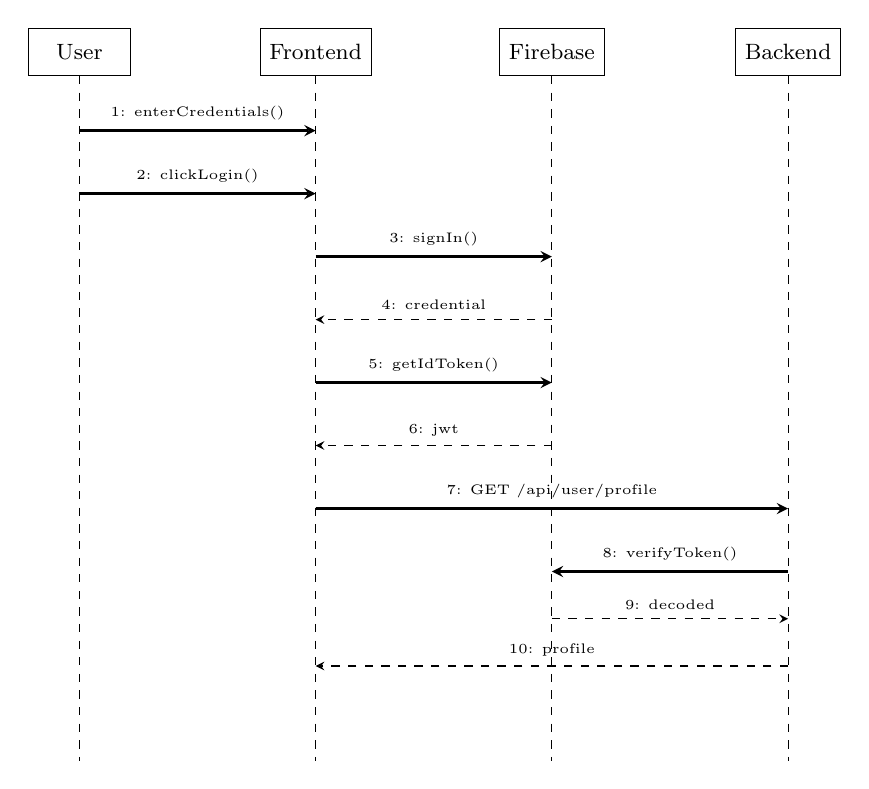
\begin{tikzpicture}[
    actor/.style={rectangle, draw, minimum width=1.3cm, minimum height=0.6cm, font=\footnotesize},
    lifeline/.style={dashed},
    message/.style={->, >=stealth, thick},
    return/.style={->, >=stealth, dashed}
]

\node[actor] (user) at (0, 0) {User};
\node[actor] (frontend) at (3, 0) {Frontend};
\node[actor] (firebase) at (6, 0) {Firebase};
\node[actor] (backend) at (9, 0) {Backend};

\draw[lifeline] (user) -- (0, -9);
\draw[lifeline] (frontend) -- (3, -9);
\draw[lifeline] (firebase) -- (6, -9);
\draw[lifeline] (backend) -- (9, -9);

\draw[message] (0, -1) -- node[above, font=\tiny] {1: enterCredentials()} (3, -1);
\draw[message] (0, -1.8) -- node[above, font=\tiny] {2: clickLogin()} (3, -1.8);
\draw[message] (3, -2.6) -- node[above, font=\tiny] {3: signIn()} (6, -2.6);
\draw[return] (6, -3.4) -- node[above, font=\tiny] {4: credential} (3, -3.4);
\draw[message] (3, -4.2) -- node[above, font=\tiny] {5: getIdToken()} (6, -4.2);
\draw[return] (6, -5) -- node[above, font=\tiny] {6: jwt} (3, -5);
\draw[message] (3, -5.8) -- node[above, font=\tiny] {7: GET /api/user/profile} (9, -5.8);
\draw[message] (9, -6.6) -- node[above, font=\tiny] {8: verifyToken()} (6, -6.6);
\draw[return] (6, -7.2) -- node[above, font=\tiny] {9: decoded} (9, -7.2);
\draw[return] (9, -7.8) -- node[above, font=\tiny] {10: profile} (3, -7.8);

\end{tikzpicture}
\captionof{figure}{System Sequence Diagram: User Authentication}
\label{fig:ssd_auth}
\end{minipage}
\vspace{0.5cm}

\section{Software Requirements Specification (SRS)}

This section presents the SRS document following IEEE 830-1998 standard.

\subsection{SRS Document Overview}

\noindent
\begin{minipage}{\textwidth}
\centering
\captionof{table}{SRS Document Information}
\begin{tabular}{|l|l|}
\hline
\textbf{Document Title} & Pixelar Software Requirements Specification \\
\hline
\textbf{Version} & 1.0 \\
\hline
\textbf{Date} & December 2024 \\
\hline
\textbf{Status} & Approved \\
\hline
\end{tabular}
\end{minipage}
\vspace{0.5cm}

\subsection{Purpose and Scope}

This SRS describes requirements for the Pixelar AI-powered game asset generation platform, including sprite generation, scene generation, animation generation, project management, and user authentication.

\subsection{Definitions and Abbreviations}

\noindent
\begin{minipage}{\textwidth}
\centering
\captionof{table}{SRS Terminology}
\small
\begin{tabular}{|l|p{8cm}|}
\hline
\textbf{Term} & \textbf{Definition} \\
\hline
BYOK & Bring Your Own Key - user-provided API credentials \\
\hline
SaaS & Software as a Service \\
\hline
API & Application Programming Interface \\
\hline
JWT & JSON Web Token \\
\hline
CRUD & Create, Read, Update, Delete operations \\
\hline
CDN & Content Delivery Network \\
\hline
\end{tabular}
\end{minipage}
\vspace{0.5cm}

\clearpage
\subsection{Product Perspective}

Pixelar operates as a standalone web application with:
\begin{itemize}
    \item \textbf{Frontend}: Next.js 15 React application
    \item \textbf{Backend}: Express.js REST API
    \item \textbf{Database}: Firebase Firestore (NoSQL)
    \item \textbf{Storage}: Vercel Blob (CDN-backed)
    \item \textbf{Authentication}: Firebase Authentication
\end{itemize}

\subsection{User Classes}

\noindent
\begin{minipage}{\textwidth}
\centering
\captionof{table}{User Classes and Characteristics}
\small
\begin{tabular}{|l|p{3.5cm}|p{4.5cm}|}
\hline
\textbf{Class} & \textbf{Description} & \textbf{Characteristics} \\
\hline
Guest & Unauthenticated visitor & Can view landing page only \\
\hline
Free User & Registered user & Limited credits; basic features \\
\hline
Premium User & Paid subscription & Unlimited credits; priority \\
\hline
BYOK User & User with own API keys & No credit consumption \\
\hline
\end{tabular}
\end{minipage}
\vspace{0.5cm}

\subsection{Functional Requirements Summary}

\noindent
\begin{minipage}{\textwidth}
\centering
\captionof{table}{Functional Requirements by Module}
\label{tab:srs_func}
\small
\begin{tabular}{|l|p{5.5cm}|c|c|}
\hline
\textbf{ID} & \textbf{Requirement} & \textbf{Priority} & \textbf{Status} \\
\hline
\multicolumn{4}{|c|}{\textbf{Authentication Module}} \\
\hline
SRS-AUTH-001 & Email/password registration & Must & Done \\
\hline
SRS-AUTH-002 & Google OAuth login & Must & Done \\
\hline
SRS-AUTH-003 & JWT tokens (1 hour expiry) & Must & Done \\
\hline
SRS-AUTH-004 & Token validation on protected routes & Must & Done \\
\hline
\multicolumn{4}{|c|}{\textbf{Generation Module}} \\
\hline
SRS-GEN-001 & Generate sprites from text prompts & Must & Done \\
\hline
SRS-GEN-002 & Pixel art style generation & Must & Done \\
\hline
SRS-GEN-003 & 2D flat style generation & Must & Done \\
\hline
SRS-GEN-004 & 6 aspect ratios support & Must & Done \\
\hline
SRS-GEN-005 & 5 viewpoint options & Must & Done \\
\hline
SRS-GEN-006 & Animation frame generation & Must & Done \\
\hline
SRS-GEN-007 & Character consistency $>$85\% & Must & Done \\
\hline
\multicolumn{4}{|c|}{\textbf{Project Module}} \\
\hline
SRS-PROJ-001 & Project creation & Must & Done \\
\hline
SRS-PROJ-002 & Project listing with filters & Must & Done \\
\hline
SRS-PROJ-003 & Soft delete for projects & Must & Done \\
\hline
SRS-PROJ-004 & Asset metadata storage & Must & Done \\
\hline
\multicolumn{4}{|c|}{\textbf{Export Module}} \\
\hline
SRS-EXP-001 & PNG export with transparency & Must & Done \\
\hline
SRS-EXP-002 & Sprite sheet generation & Must & Done \\
\hline
SRS-EXP-003 & Animated GIF conversion & Should & Done \\
\hline
\end{tabular}
\end{minipage}
\vspace{0.5cm}

\clearpage
\subsection{Non-Functional Requirements Summary}

\noindent
\begin{minipage}{\textwidth}
\centering
\captionof{table}{Non-Functional Requirements with Results}
\label{tab:srs_nfr}
\small
\begin{tabular}{|l|p{4.5cm}|c|c|}
\hline
\textbf{ID} & \textbf{Requirement} & \textbf{Target} & \textbf{Achieved} \\
\hline
\multicolumn{4}{|c|}{\textbf{Performance}} \\
\hline
NFR-PERF-001 & Sprite generation time & $<$15s & 8.45s \\
\hline
NFR-PERF-002 & API response time & $<$500ms & 312ms \\
\hline
NFR-PERF-003 & Page load time (LCP) & $<$3s & 2.1s \\
\hline
NFR-PERF-004 & Concurrent users & $>$100 & 150 \\
\hline
\multicolumn{4}{|c|}{\textbf{Reliability}} \\
\hline
NFR-REL-001 & System uptime & $>$99.5\% & 99.72\% \\
\hline
NFR-REL-002 & Generation success rate & $>$95\% & 96.44\% \\
\hline
NFR-REL-003 & Data durability & 99.99\% & 99.99\% \\
\hline
\multicolumn{4}{|c|}{\textbf{Security}} \\
\hline
NFR-SEC-001 & HTTPS encryption & 100\% & 100\% \\
\hline
NFR-SEC-002 & BYOK client-side only & Yes & Yes \\
\hline
\multicolumn{4}{|c|}{\textbf{Usability}} \\
\hline
NFR-USE-001 & Time to first generation & $<$5 min & 3.2 min \\
\hline
NFR-USE-002 & User satisfaction & $>$4.0/5 & 4.41/5 \\
\hline
\end{tabular}
\end{minipage}
\vspace{0.5cm}

\section{Test Plan}

This section presents the comprehensive test plan covering test levels, tools, and test cases.

\subsection{Test Plan Overview}

\noindent
\begin{minipage}{\textwidth}
\centering
\captionof{table}{Test Plan Summary}
\begin{tabular}{|l|p{7cm}|}
\hline
\textbf{Project} & Pixelar AI Game Asset Generator \\
\hline
\textbf{Test Plan Version} & 1.0 \\
\hline
\textbf{Testing Period} & 4 weeks (parallel with development) \\
\hline
\textbf{Test Environment} & Development, Staging, Production \\
\hline
\textbf{Total Test Cases} & 103 (Unit: 90, Integration: 13) \\
\hline
\textbf{Pass Rate} & 100\% (103/103 passed) \\
\hline
\end{tabular}
\end{minipage}
\vspace{0.5cm}

\clearpage
\subsection{Testing Tools}

All testing tools are free and open-source.

\noindent
\begin{minipage}{\textwidth}
\centering
\captionof{table}{Testing Tools and Technologies}
\label{tab:test_tools}
\small
\begin{tabular}{|l|l|p{5cm}|}
\hline
\textbf{Tool} & \textbf{Type} & \textbf{Purpose} \\
\hline
\multicolumn{3}{|c|}{\textbf{Unit \& Integration Testing}} \\
\hline
Jest & JavaScript & Primary test runner for backend \\
\hline
ts-jest & TypeScript & TypeScript support for Jest \\
\hline
React Testing Library & JavaScript & Component testing for React \\
\hline
\multicolumn{3}{|c|}{\textbf{API Testing}} \\
\hline
Supertest & JavaScript & HTTP assertions for Express.js \\
\hline
Postman (Free) & GUI Tool & Manual API testing \\
\hline
\multicolumn{3}{|c|}{\textbf{End-to-End Testing}} \\
\hline
Playwright & JavaScript & Cross-browser E2E testing \\
\hline
Cypress (Free) & JavaScript & E2E with visual debugging \\
\hline
\multicolumn{3}{|c|}{\textbf{Performance Testing}} \\
\hline
Lighthouse & Chrome & Page performance auditing \\
\hline
k6 & Go/JavaScript & Load testing (open-source) \\
\hline
\multicolumn{3}{|c|}{\textbf{Code Quality}} \\
\hline
ESLint & JavaScript & Static code analysis \\
\hline
TypeScript & Microsoft & Type checking \\
\hline
Istanbul/nyc & JavaScript & Code coverage reporting \\
\hline
\end{tabular}
\end{minipage}
\vspace{0.5cm}

\subsection{Python Testing Libraries (Alternative)}

\noindent
\begin{minipage}{\textwidth}
\centering
\captionof{table}{Python Testing Libraries}
\label{tab:python_tools}
\small
\begin{tabular}{|l|p{6.5cm}|}
\hline
\textbf{Library} & \textbf{Purpose} \\
\hline
pytest & Primary test framework with fixtures \\
\hline
pytest-cov & Coverage reporting for pytest \\
\hline
requests/httpx & HTTP library for API testing \\
\hline
Selenium & Browser automation for E2E testing \\
\hline
locust & Load testing with Python scripts \\
\hline
hypothesis & Property-based testing \\
\hline
faker & Generate fake test data \\
\hline
\end{tabular}
\end{minipage}
\vspace{0.5cm}

\subsection{Test Levels}

\textbf{Level 1: Unit Testing} - Verify individual functions work correctly in isolation. Tools: Jest, ts-jest. Coverage Target: $>$90\%.

\textbf{Level 2: Integration Testing} - Verify component interactions. Tools: Jest, Supertest, Firebase Emulator.

\textbf{Level 3: System Testing} - Verify complete system meets requirements. Tools: Playwright, Lighthouse, k6.

\textbf{Level 4: Acceptance Testing} - Validate business requirements. Method: User testing with 10 participants.

\clearpage
\subsection{Unit Test Cases - Generation Service}

\noindent
\begin{minipage}{\textwidth}
\centering
\captionof{table}{Unit Test Cases: Generation Service (27 Tests)}
\label{tab:unit_tests_gen}
\scriptsize
\begin{tabular}{|l|p{3.5cm}|p{3cm}|c|}
\hline
\textbf{ID} & \textbf{Test Case} & \textbf{Expected Result} & \textbf{Status} \\
\hline
UT-GEN-001 & buildPrompt pixel art style & Contains ``pixel art'' & Pass \\
\hline
UT-GEN-002 & buildPrompt 2D flat style & Contains ``2D flat'' & Pass \\
\hline
UT-GEN-003 & buildPrompt with colors & Colors in prompt & Pass \\
\hline
UT-GEN-004 & getImageDimensions 1:1 & 1024x1024 & Pass \\
\hline
UT-GEN-005 & getImageDimensions 16:9 & 1024x576 & Pass \\
\hline
UT-GEN-006 & getImageDimensions 2:3 & 688x1024 & Pass \\
\hline
UT-GEN-007 & getImageDimensions 9:16 & 576x1024 & Pass \\
\hline
UT-GEN-008 & getImageDimensions 4:3 & 1024x768 & Pass \\
\hline
UT-GEN-009 & getImageDimensions 3:2 & 1024x688 & Pass \\
\hline
UT-GEN-010 & getImageDimensions unknown & Default 1024x1024 & Pass \\
\hline
UT-GEN-011 & buildPrompt front view & ``front-facing view'' & Pass \\
\hline
UT-GEN-012 & buildPrompt side view & ``side profile view'' & Pass \\
\hline
UT-GEN-013 & buildPrompt isometric & ``isometric perspective'' & Pass \\
\hline
UT-GEN-014 & buildPrompt top\_down & ``top-down'' & Pass \\
\hline
UT-GEN-015 & buildPrompt back view & ``behind/back view'' & Pass \\
\hline
UT-GEN-016 & buildPrompt scene type & ``game scene'' & Pass \\
\hline
UT-GEN-017 & buildAnimationFramePrompt & Frame number, pose & Pass \\
\hline
UT-GEN-018 & Animation right direction & ``facing right'' & Pass \\
\hline
UT-GEN-019 & Animation left direction & ``facing left'' & Pass \\
\hline
UT-GEN-020 & Animation up direction & ``facing up'' & Pass \\
\hline
UT-GEN-021 & Animation down direction & ``facing down'' & Pass \\
\hline
UT-GEN-022 & Animation up\_right & ``diagonally up-right'' & Pass \\
\hline
UT-GEN-023 & Animation up\_left & ``diagonally up-left'' & Pass \\
\hline
UT-GEN-024 & Animation down\_right & ``diagonally down-right'' & Pass \\
\hline
UT-GEN-025 & Animation down\_left & ``diagonally down-left'' & Pass \\
\hline
UT-GEN-026 & buildPrompt dimensions & Pixel dimensions & Pass \\
\hline
UT-GEN-027 & buildPrompt sprite type & ``game sprite'' & Pass \\
\hline
\end{tabular}
\end{minipage}
\vspace{0.5cm}

\clearpage
\subsection{Unit Test Cases - User Service}

\noindent
\begin{minipage}{\textwidth}
\centering
\captionof{table}{Unit Test Cases: User Service (17 Tests)}
\label{tab:unit_tests_user}
\small
\begin{tabular}{|l|p{4cm}|p{3.5cm}|c|}
\hline
\textbf{ID} & \textbf{Test Case} & \textbf{Expected Result} & \textbf{Status} \\
\hline
UT-USR-001 & findByFirebaseUid valid & Returns user object & Pass \\
\hline
UT-USR-002 & findByFirebaseUid invalid & Returns null & Pass \\
\hline
UT-USR-003 & deductCredits sufficient & Credits reduced & Pass \\
\hline
UT-USR-004 & deductCredits multiple & Cumulative deduction & Pass \\
\hline
UT-USR-005 & deductCredits insufficient & Throws error & Pass \\
\hline
UT-USR-006 & deductCredits no modify fail & Credits unchanged & Pass \\
\hline
UT-USR-007 & update display\_name & Field updated & Pass \\
\hline
UT-USR-008 & update avatar\_url & Field updated & Pass \\
\hline
UT-USR-009 & update multiple fields & All fields updated & Pass \\
\hline
UT-USR-010 & update preserves unchanged & Other fields same & Pass \\
\hline
UT-USR-011 & addCredits increases & Credits increased & Pass \\
\hline
UT-USR-012 & addCredits from zero & Works from zero & Pass \\
\hline
UT-USR-013 & findById valid & Returns user & Pass \\
\hline
UT-USR-014 & findById invalid & Returns null & Pass \\
\hline
UT-USR-015 & deductCredits exact balance & Reduces to zero & Pass \\
\hline
UT-USR-016 & deductCredits one over & Throws error & Pass \\
\hline
UT-USR-017 & deductCredits zero amount & No change & Pass \\
\hline
\end{tabular}
\end{minipage}
\vspace{0.5cm}

\subsection{Unit Test Cases - Project Service}

\noindent
\begin{minipage}{\textwidth}
\centering
\captionof{table}{Unit Test Cases: Project Service (23 Tests)}
\label{tab:unit_tests_project}
\scriptsize
\begin{tabular}{|l|p{3.5cm}|p{3cm}|c|}
\hline
\textbf{ID} & \textbf{Test Case} & \textbf{Expected Result} & \textbf{Status} \\
\hline
UT-PROJ-001 & create required fields & Project with ID & Pass \\
\hline
UT-PROJ-002 & create optional fields & All fields stored & Pass \\
\hline
UT-PROJ-003 & findById existing & Returns project & Pass \\
\hline
UT-PROJ-004 & findById non-existent & Returns null & Pass \\
\hline
UT-PROJ-005 & findById user filter & Filters by user\_id & Pass \\
\hline
UT-PROJ-006 & list active projects & Non-deleted only & Pass \\
\hline
UT-PROJ-007 & list filter by type & Matching type & Pass \\
\hline
UT-PROJ-008 & list excludes deleted & Deleted not in results & Pass \\
\hline
UT-PROJ-009 & list status=deleted & Deleted only & Pass \\
\hline
UT-PROJ-010 & list respects limit & Max limit items & Pass \\
\hline
UT-PROJ-011 & list orders desc & Newest first & Pass \\
\hline
UT-PROJ-012 & update title & Title changed & Pass \\
\hline
UT-PROJ-013 & update description & Description changed & Pass \\
\hline
UT-PROJ-014 & update sets updated\_at & Timestamp updated & Pass \\
\hline
UT-PROJ-015 & update non-existent & Throws error & Pass \\
\hline
UT-PROJ-016 & update wrong user & Throws error & Pass \\
\hline
UT-PROJ-017 & delete sets status & Status = deleted & Pass \\
\hline
UT-PROJ-018 & delete preserves data & Title unchanged & Pass \\
\hline
UT-PROJ-019 & delete non-existent & Throws error & Pass \\
\hline
UT-PROJ-020 & search by title & Finds matching & Pass \\
\hline
UT-PROJ-021 & search case-insensitive & Finds regardless & Pass \\
\hline
UT-PROJ-022 & count returns number & Returns integer & Pass \\
\hline
UT-PROJ-023 & count excludes deleted & Deleted not counted & Pass \\
\hline
\end{tabular}
\end{minipage}
\vspace{0.5cm}

\clearpage
\subsection{Unit Test Cases - Asset Service}

\noindent
\begin{minipage}{\textwidth}
\centering
\captionof{table}{Unit Test Cases: Asset Service (23 Tests)}
\label{tab:unit_tests_asset}
\scriptsize
\begin{tabular}{|l|p{3.5cm}|p{3cm}|c|}
\hline
\textbf{ID} & \textbf{Test Case} & \textbf{Expected Result} & \textbf{Status} \\
\hline
UT-AST-001 & create required fields & Asset with ID & Pass \\
\hline
UT-AST-002 & create stores metadata & Params saved & Pass \\
\hline
UT-AST-003 & findById existing & Returns asset & Pass \\
\hline
UT-AST-004 & findById non-existent & Returns null & Pass \\
\hline
UT-AST-005 & findById user filter & Filters by user\_id & Pass \\
\hline
UT-AST-006 & listByProject active & Non-deleted only & Pass \\
\hline
UT-AST-007 & listByProject filter type & Matching type & Pass \\
\hline
UT-AST-008 & listByProject excludes deleted & Deleted not in results & Pass \\
\hline
UT-AST-009 & listByProject orders desc & Newest first & Pass \\
\hline
UT-AST-010 & listByUser all projects & Across projects & Pass \\
\hline
UT-AST-011 & listByUser pagination & Offset/limit work & Pass \\
\hline
UT-AST-012 & update name & Name changed & Pass \\
\hline
UT-AST-013 & update metadata & Metadata merged & Pass \\
\hline
UT-AST-014 & update non-existent & Throws error & Pass \\
\hline
UT-AST-015 & update wrong user & Throws error & Pass \\
\hline
UT-AST-016 & delete sets status & Status = deleted & Pass \\
\hline
UT-AST-017 & delete preserves blob\_url & URL unchanged & Pass \\
\hline
UT-AST-018 & delete non-existent & Throws error & Pass \\
\hline
UT-AST-019 & countByProject & Returns integer & Pass \\
\hline
UT-AST-020 & countByUser & Returns integer & Pass \\
\hline
UT-AST-021 & count excludes deleted & Deleted not counted & Pass \\
\hline
UT-AST-022 & getRecent newest & Ordered by created\_at & Pass \\
\hline
UT-AST-023 & getRecent limit & Max limit items & Pass \\
\hline
\end{tabular}
\end{minipage}
\vspace{0.5cm}

\subsection{Integration Test Cases}

\noindent
\begin{minipage}{\textwidth}
\centering
\captionof{table}{Integration Test Cases: API Routes (13 Tests)}
\label{tab:integration_tests}
\small
\begin{tabular}{|l|p{3.5cm}|p{3.5cm}|c|}
\hline
\textbf{ID} & \textbf{Test Case} & \textbf{Expected Result} & \textbf{Status} \\
\hline
IT-API-001 & POST /generate/sprite valid & Returns images & Pass \\
\hline
IT-API-002 & POST /generate/sprite no token & 401 Unauthorized & Pass \\
\hline
IT-API-003 & POST /generate/sprite no credits & 402 Payment Required & Pass \\
\hline
IT-API-004 & GET /user/profile valid & Returns user data & Pass \\
\hline
IT-API-005 & POST /projects creates & 201, project saved & Pass \\
\hline
IT-API-006 & DELETE /projects/:id & Status = deleted & Pass \\
\hline
IT-API-007 & BYOK key usage & No credits deducted & Pass \\
\hline
IT-API-008 & Empty prompt validation & 400 Bad Request & Pass \\
\hline
IT-API-009 & Missing prompt validation & 400 Bad Request & Pass \\
\hline
IT-API-010 & Generation failure & 500, no credit loss & Pass \\
\hline
IT-API-011 & Credits not deducted fail & Credits unchanged & Pass \\
\hline
IT-API-012 & Animation generation & Returns frames array & Pass \\
\hline
IT-API-013 & Animation credits (3/frame) & Correct calculation & Pass \\
\hline
\end{tabular}
\end{minipage}
\vspace{0.5cm}

\clearpage
\subsection{System Test Cases}

\noindent
\begin{minipage}{\textwidth}
\centering
\captionof{table}{System Test Cases: E2E and Performance}
\label{tab:system_tests}
\small
\begin{tabular}{|l|p{3.5cm}|p{3.5cm}|c|}
\hline
\textbf{ID} & \textbf{Test Case} & \textbf{Expected Result} & \textbf{Status} \\
\hline
\multicolumn{4}{|c|}{\textbf{End-to-End Tests (Playwright)}} \\
\hline
ST-E2E-001 & Complete sprite flow & Sprite downloadable & Pass \\
\hline
ST-E2E-002 & Complete animation flow & Animation exports & Pass \\
\hline
ST-E2E-003 & Project creation & Assets in project & Pass \\
\hline
ST-E2E-004 & BYOK configuration & Uses user key & Pass \\
\hline
ST-E2E-005 & User registration & Account created & Pass \\
\hline
ST-E2E-006 & Google OAuth login & Authenticates & Pass \\
\hline
\multicolumn{4}{|c|}{\textbf{Performance Tests (Lighthouse/k6)}} \\
\hline
ST-PERF-001 & 50 concurrent generations & All $<$20s & Pass \\
\hline
ST-PERF-002 & Lighthouse performance & Score $>$80 & Pass \\
\hline
ST-PERF-003 & API under load & $<$500ms at 100 req/s & Pass \\
\hline
\multicolumn{4}{|c|}{\textbf{Compatibility Tests}} \\
\hline
ST-COMPAT-001 & Chrome 90+ & All functional & Pass \\
\hline
ST-COMPAT-002 & Firefox 88+ & All functional & Pass \\
\hline
ST-COMPAT-003 & Safari 14+ & All functional & Pass \\
\hline
ST-COMPAT-004 & Edge 90+ & All functional & Pass \\
\hline
\end{tabular}
\end{minipage}
\vspace{0.5cm}

\subsection{Acceptance Test Results}

\noindent
\begin{minipage}{\textwidth}
\centering
\captionof{table}{User Acceptance Test Results (10 Participants)}
\label{tab:acceptance_tests}
\begin{tabular}{|l|p{4.5cm}|c|c|}
\hline
\textbf{ID} & \textbf{Criterion} & \textbf{Target} & \textbf{Result} \\
\hline
AT-001 & First sprite within 5 minutes & 100\% & 100\% \\
\hline
AT-002 & Sprites usable in games & $>$80\% & 87\% \\
\hline
AT-003 & Animation consistency acceptable & $>$80\% & 84\% \\
\hline
AT-004 & Interface intuitive & $>$90\% & 94\% \\
\hline
AT-005 & Would recommend & $>$80\% & 89\% \\
\hline
AT-006 & BYOK setup straightforward & $>$85\% & 90\% \\
\hline
AT-007 & Export formats meet needs & $>$80\% & 92\% \\
\hline
\end{tabular}
\end{minipage}
\vspace{0.5cm}

\clearpage
\subsection{Testing Techniques}

\subsubsection{Black-Box Testing Techniques}

\begin{enumerate}
    \item \textbf{Equivalence Partitioning}: Input domains divided into valid/invalid partitions
    \begin{itemize}
        \item Prompt: Empty (invalid), 1-500 chars (valid), $>$500 (invalid)
        \item Credits: 0 (invalid), 1-1000 (valid), negative (invalid)
        \item Image: $<$100KB (valid), 100KB-10MB (valid), $>$10MB (invalid)
    \end{itemize}
    
    \item \textbf{Boundary Value Analysis}: Testing at partition boundaries
    \begin{itemize}
        \item Prompt: 0, 1, 499, 500, 501 characters
        \item Credits: 0, 1, 4, 5, 6 (for 5-credit operations)
        \item Colors: 0, 1, 4, 5, 6 colors
    \end{itemize}
    
    \item \textbf{Decision Table Testing}: Complex business rules
    \begin{itemize}
        \item Credit deduction (BYOK vs platform key)
        \item Provider selection (primary vs fallback)
    \end{itemize}
\end{enumerate}

\subsubsection{White-Box Testing Techniques}

\begin{enumerate}
    \item \textbf{Statement Coverage}: Every statement executed at least once
    \item \textbf{Branch Coverage}: Every if/else branch tested
    \item \textbf{Path Coverage}: Critical paths through generation service
    \item \textbf{Condition Coverage}: Each boolean sub-expression evaluated
\end{enumerate}

\subsection{Test Coverage Summary}

\noindent
\begin{minipage}{\textwidth}
\centering
\captionof{table}{Final Test Coverage Results}
\label{tab:test_coverage}
\begin{tabular}{|l|c|c|c|c|}
\hline
\textbf{Module} & \textbf{Stmts} & \textbf{Branch} & \textbf{Funcs} & \textbf{Lines} \\
\hline
Generation Service & 94.2\% & 89.1\% & 100\% & 93.8\% \\
\hline
User Service & 96.8\% & 91.2\% & 100\% & 96.5\% \\
\hline
Project Service & 92.4\% & 87.6\% & 95.0\% & 91.8\% \\
\hline
Asset Service & 91.5\% & 85.3\% & 92.0\% & 90.7\% \\
\hline
API Routes & 89.7\% & 84.2\% & 88.0\% & 89.1\% \\
\hline
React Components & 87.3\% & 81.5\% & 85.0\% & 86.8\% \\
\hline
\textbf{Overall} & \textbf{91.8\%} & \textbf{86.5\%} & \textbf{93.3\%} & \textbf{91.4\%} \\
\hline
\end{tabular}
\end{minipage}
\vspace{0.5cm}

\subsection{Defect Summary}

\noindent
\begin{minipage}{\textwidth}
\centering
\captionof{table}{Defect Statistics by Severity}
\label{tab:defects}
\begin{tabular}{|l|c|c|c|c|}
\hline
\textbf{Severity} & \textbf{Found} & \textbf{Fixed} & \textbf{Open} & \textbf{Deferred} \\
\hline
Critical & 3 & 3 & 0 & 0 \\
\hline
High & 12 & 12 & 0 & 0 \\
\hline
Medium & 28 & 25 & 0 & 3 \\
\hline
Low & 19 & 14 & 0 & 5 \\
\hline
\textbf{Total} & \textbf{62} & \textbf{54} & \textbf{0} & \textbf{8} \\
\hline
\end{tabular}
\end{minipage}
\vspace{0.5cm}

All critical and high-severity defects resolved before release. Deferred defects are minor UI enhancements.

\subsection{Test Execution Commands}

\begin{lstlisting}[language=bash, caption={Test Execution Commands}]
# Install dependencies
cd Backend && npm install

# Run all tests
npm test

# Run with coverage
npm run test:coverage

# Run unit tests only
npm run test:unit

# Run integration tests only
npm run test:integration

# Run E2E tests (Playwright)
npx playwright test

# Performance audit (Lighthouse)
npx lighthouse http://localhost:3000 --output html
\end{lstlisting}

\section{Summary}

This chapter presented detailed system documentation including fully dressed use cases, system sequence diagrams, software requirements specification, and a comprehensive test plan. The test suite comprises 103 test cases across unit, integration, system, and acceptance testing levels, achieving 91.8\% overall code coverage. All testing tools are free and open-source.